Today I am working on formalizing what I saw on the 13th. 

Consider the Kunz coordinates associated to a numerical semigroup with multiplicity $m=3$. For $Ap(S) = \{ 3, 3k_1+1, 3k_2+2\}$ we have the associated coordinates $(k_1, k_2).$

If $S \to (k_1, k_2)$ then the children of $S$ will be 
\begin{itemize}
    \item $(k_1 + 1, k_2)$ when $k_2 + 1 \leq k_1 < 2k_2 + 1$,
    \item $(k_1, k_2 + 1)$ when $k_1 \leq k_2 < 2k_1$.
\end{itemize}
Note: If $k_1=k_2$ or $k_1 = k_2 + 1$ both $(k_1 + 1, k_2)$ and $(k_1, k_2 + 1)$ will be children. If $k_1 = 2k+1$ or $k_2 = 2k_1$ there will be no children.

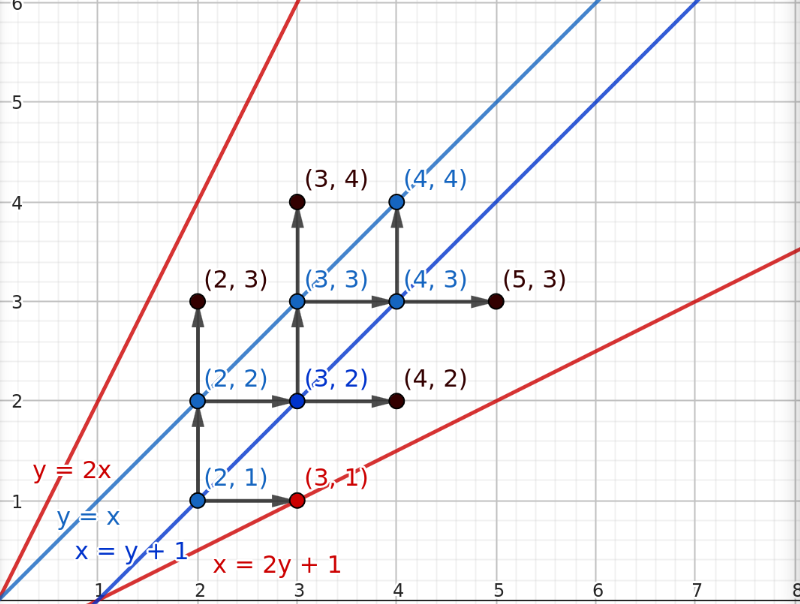
\includegraphics[scale=0.3]{Max/images/Screenshot from 2024-07-15 13-01-52.png}